\documentclass[border=10pt]{standalone}
\usepackage[svgnames]{xcolor}
\usepackage{amsmath}
\usepackage{pgfplots}
\pgfplotsset{compat=newest}
\usepackage[sfdefault]{FiraSans}
\usepackage{FiraMono}
\renewcommand*\familydefault{\sfdefault}
\begin{document}
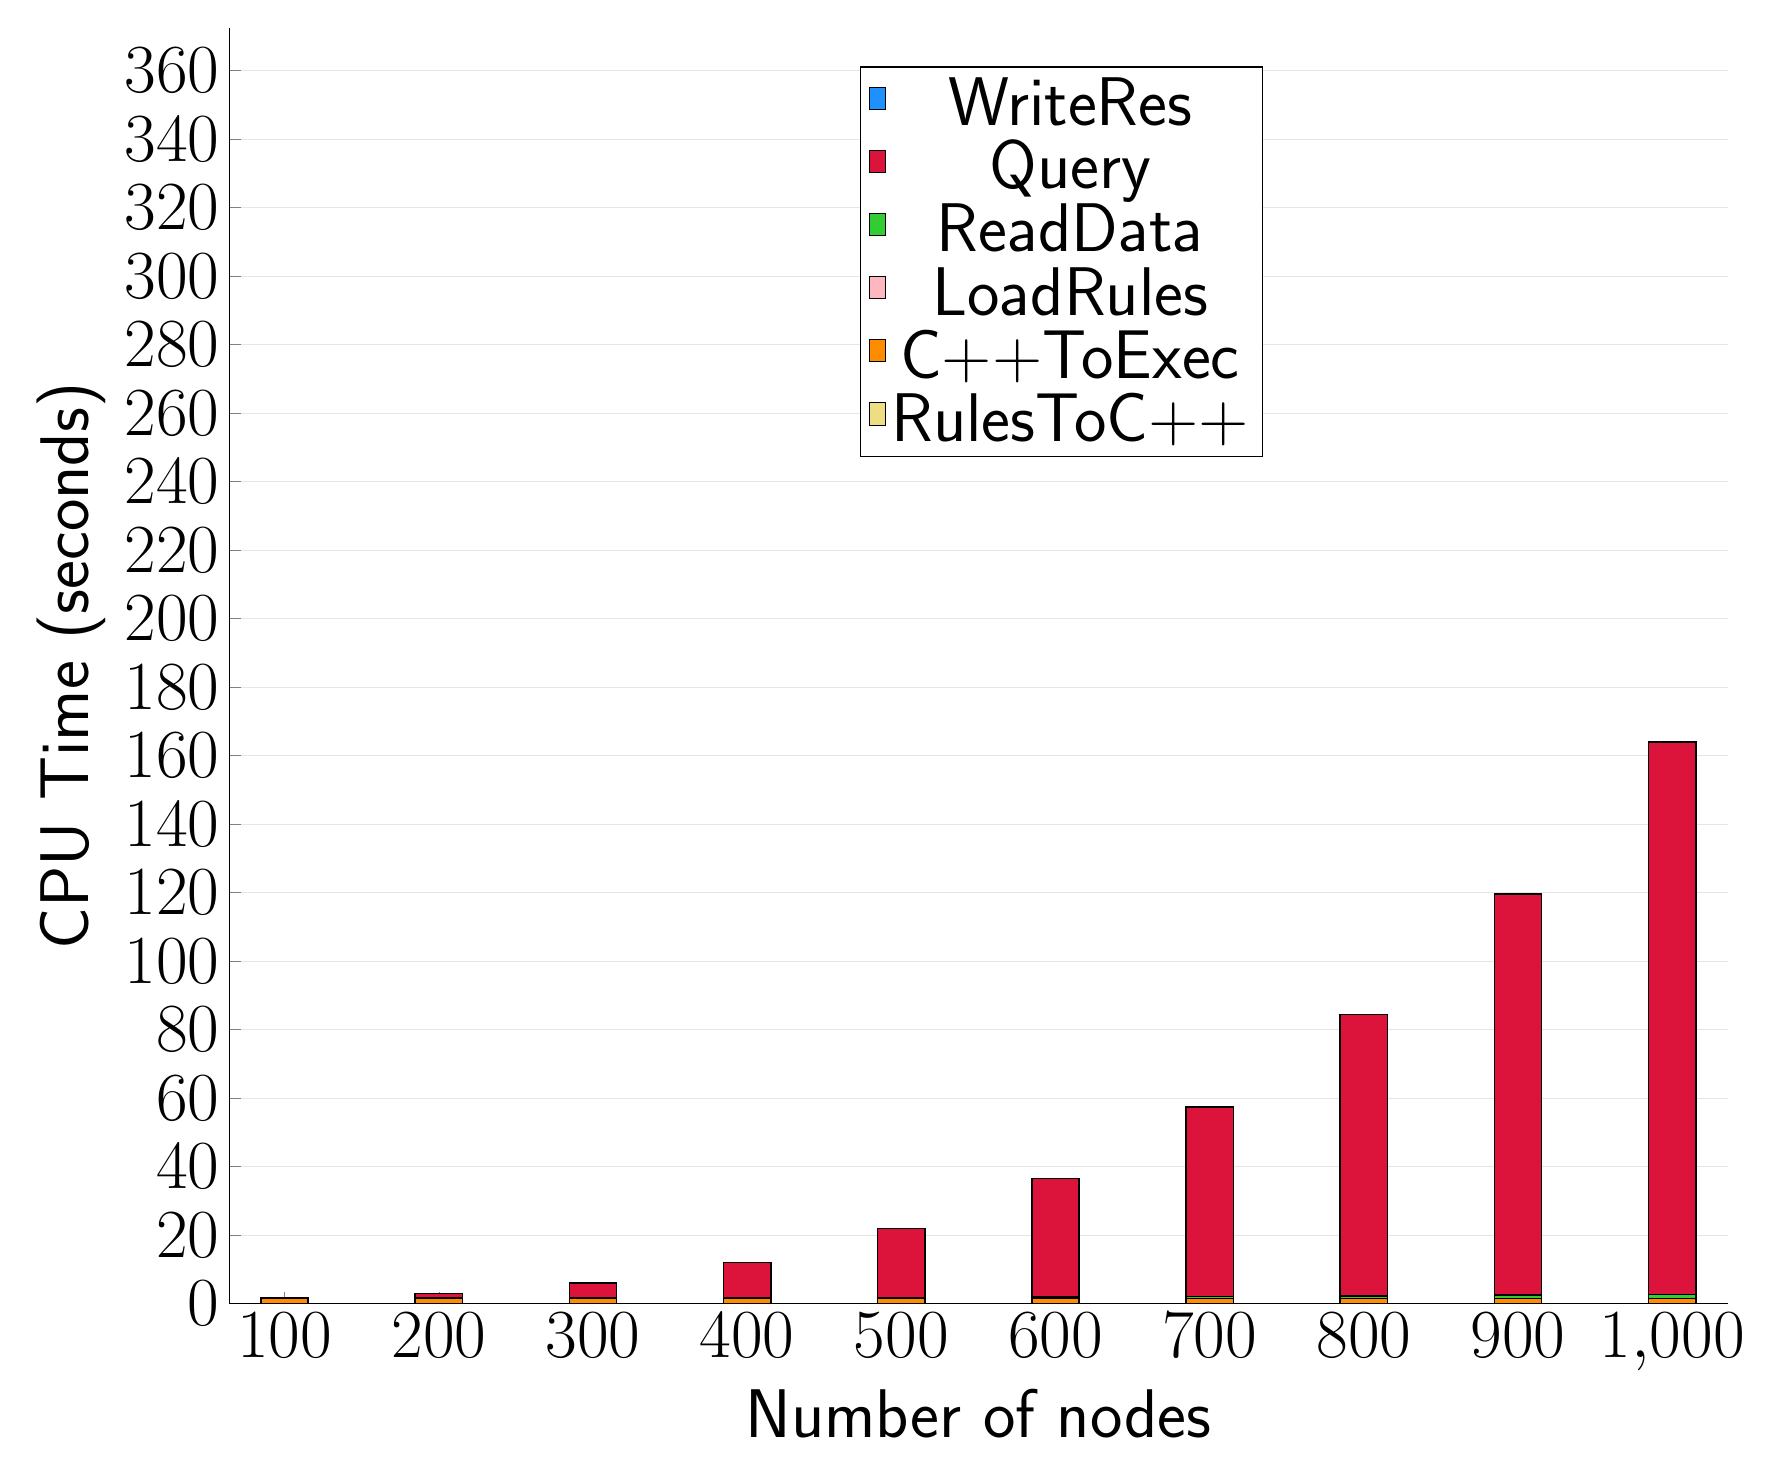
\begin{tikzpicture}
\begin{axis}[
   ybar stacked,
   width=1.7\textwidth,
   bar width=0.6cm,
   ymajorgrids, tick align=inside,
   major grid style={draw=gray!20},
   xtick=data,
   ymin=0, ymax=372.4108,
   axis x line*=bottom,
   axis y line*=left,
   enlarge x limits=0.04,
   legend style={
       at={(0.69, 0.97)},
       anchor=north east,
       legend columns=1,
       font=\Huge,
   },
   ylabel={CPU Time (seconds)},
   xlabel={Number of nodes},
   label style={font=\Huge},
   tick label style={font=\Huge},
]
\addlegendimage{fill=DodgerBlue, draw=black, line width=0.2pt}
\addlegendentry{WriteRes}
\addlegendimage{fill=Crimson, draw=black, line width=0.2pt}
\addlegendentry{Query}
\addlegendimage{fill=LimeGreen, draw=black, line width=0.2pt}
\addlegendentry{ReadData}
\addlegendimage{fill=LightPink, draw=black, line width=0.2pt}
\addlegendentry{LoadRules}
\addlegendimage{fill=DarkOrange, draw=black, line width=0.2pt}
\addlegendentry{C++ToExec}
\addlegendimage{fill=LightGoldenrod, draw=black, line width=0.2pt}
\addlegendentry{RulesToC++}
\addplot +[fill=LightGoldenrod, draw=black, line width=0.55pt] coordinates {
(100, 0.010000000000000002)
(200, 0.008000000000000002)
(300, 0.008000000000000002)
(400, 0.006000000000000001)
(500, 0.006000000000000001)
(600, 0.006000000000000001)
(700, 0.004000000000000001)
(800, 0.004000000000000001)
(900, 0.0020000000000000005)
(1000, 0.0020000000000000005)
};
\addplot +[fill=DarkOrange, draw=black, line width=0.55pt] coordinates {
(100, 1.5320000000000003)
(200, 1.528)
(300, 1.5300000000000002)
(400, 1.53)
(500, 1.528)
(600, 1.528)
(700, 1.528)
(800, 1.53)
(900, 1.524)
(1000, 1.512)
};
\addplot +[fill=LightPink, draw=black, line width=0.55pt] coordinates {
(100, 0.0001428)
(200, 0.00014419999999999998)
(300, 0.0001436)
(400, 0.000141)
(500, 0.0001448)
(600, 0.00015500000000000003)
(700, 0.00014159999999999997)
(800, 0.00014780000000000001)
(900, 0.000186)
(1000, 0.0001516)
};
\addplot +[fill=LimeGreen, draw=black, line width=0.55pt] coordinates {
(100, 0.023932200000000004)
(200, 0.065429)
(300, 0.1240976)
(400, 0.2036384)
(500, 0.3061654)
(600, 0.43665699999999996)
(700, 0.5848946)
(800, 0.7599658)
(900, 0.960262)
(1000, 1.1805720000000002)
};
\addplot +[fill=Crimson, draw=black, line width=0.55pt] coordinates {
(100, 0.1770184)
(200, 1.303504)
(300, 4.333464)
(400, 10.3077)
(500, 20.13256)
(600, 34.55210000000001)
(700, 55.3261)
(800, 82.13485999999999)
(900, 117.04720000000002)
(1000, 161.3684)
};
\addplot +[fill=DodgerBlue, draw=black, line width=0.55pt] coordinates {
(100, 0.00022519999999999997)
(200, 0.00033239999999999995)
(300, 0.00037480000000000006)
(400, 0.0004188)
(500, 0.0003574)
(600, 0.0004328)
(700, 0.00046960000000000003)
(800, 0.0004648)
(900, 0.0004634)
(1000, 0.0005128)
};
\end{axis}
\end{tikzpicture}

\end{document}
